\documentclass[
11pt, % Set the default font size, options include: 8pt, 9pt, 10pt, 11pt, 12pt, 14pt, 17pt, 20pt
%t, % Uncomment to vertically align all slide content to the top of the slide, rather than the default centered
%aspectratio=169, % Uncomment to set the aspect ratio to a 16:9 ratio which matches the aspect ratio of 1080p and 4K screens and projectors
]{beamer}

\graphicspath{{Images/}{./}} % Specifies where to look for included images (trailing slash required)

\usepackage{todonotes}
\usepackage{graphicx}
\usepackage{xcolor}
\usepackage{subfig}
%%\usepackage[noend]{algpseudocode}


\usepackage{algorithm}
\usepackage{algorithmic}

\usepackage{blkarray}
\usepackage{amsmath}
\usepackage{xspace}
\usepackage{float}


\usepackage{tikz}
\usetikzlibrary{matrix, decorations, patterns, positioning, shapes, calc, intersections, arrows, fit}

\usetikzlibrary{patterns}
\usetikzlibrary{fit,calc,positioning,decorations.pathreplacing,matrix,3d, hobby}

\usepackage{booktabs} % Allows the use of \toprule, \midrule and \bottomrule for better rules in tables


\newcommand{\brown}[1]{{\color{brown} #1 }}

%% Colors from https://latexcolor.com/
\definecolor{pastelviolet}{rgb}{0.8, 0.6, 0.79}
\definecolor{babyblueeyes}{rgb}{0.63, 0.79, 0.95}
\definecolor{pastelyellow}{rgb}{0.99, 0.99, 0.59}
\definecolor{pastelgreen}{rgb}{0.47, 0.87, 0.47}
\definecolor{pastelred}{rgb}{1.0, 0.41, 0.38}
\colorlet{patternblue}{blue!60}


\colorlet{darkred}{red!80!black}
\colorlet{darkblue}{blue!80!black}
\newcommand<>{\darkred}[1]{{\color{darkred}{#1}}}
\newcommand<>{\darkblue}[1]{{\color#2{blue!50!black!100}{#1}}}

\usetheme{Madrid}





%----------------------------------------------------------------------------------------
%	PRESENTATION INFORMATION
%----------------------------------------------------------------------------------------

\title[collective communication]{Collective communication costs in MPI} % The short title in the optional parameter appears at the bottom of every slide, the full title in the main parameter is only on the title page

%\subtitle{Optional Subtitle} % Presentation subtitle, remove this command if a subtitle isn't required

\author[Suraj Kumar]{Suraj Kumar} % Presenter name(s), the optional parameter can contain a shortened version to appear on the bottom of every slide, while the main parameter will appear on the title slide

\institute[Inria \& ENS Lyon]{Inria \& ENS Lyon \\ \smallskip Email:\textit{suraj.kumar@inria.fr}} % Your institution, the optional parameter can be used for the institution shorthand and will appear on the bottom of every slide after author names, while the required parameter is used on the title slide and can include your email address or additional information on separate lines

\date[CR12]{CR12: September 2023\\ \smallskip\small https://surakuma.github.io/courses/daamtc.html} % Presentation date or conference/meeting name, the optional parameter can contain a shortened version to appear on the bottom of every slide, while the required parameter value is output to the title slide

%----------------------------------------------------------------------------------------

\begin{document}
	
	%----------------------------------------------------------------------------------------
	%	TITLE SLIDE
	%----------------------------------------------------------------------------------------
	
	\begin{frame}
		\titlepage % Output the title slide, automatically created using the text entered in the PRESENTATION INFORMATION block above
	\end{frame}


\begin{frame}{Cost model}
	\begin{itemize}
		\item The links of the network are bidirectional
		\item Each process can send and receive at-most one message at the same time
		\item Time taken to send a message with $n$ bytes between any two nodes --  $T= \alpha + n\beta$
		\begin{itemize}
			\item $\alpha$: latency cost per message, $\beta$: transfer time per byte
		\end{itemize}
		\item In case of reduction operation, $\gamma$: computation cost per byte
		\item $P$ is the total number of processes 		
	\end{itemize}
\end{frame}

\begin{frame}{Allgather}
\begin{minipage}{0.45\linewidth}
	\begin{center}
		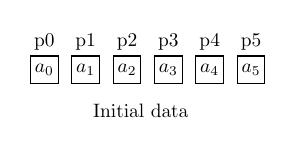
\begin{tikzpicture}[scale=0.35, every node/.style={transform shape}]
		
		%//starting at (0,0)
		
		\foreach \x in {0,1,2,3,4, 5}
		{
		\draw (1.5*\x, 0) -- ++(1, 0) -- ++(0,1) -- ++(-1,0) -- cycle;
		\node [scale=2] at (1.5*\x+0.5, 0.5) {$a_\x$};
		}
		
		
		\foreach \x in {0,1,2,3,4, 5}
		\node [scale=2] at (1.5*\x+0.5 , 1.5) {p\x};
		
		\node [scale=2] at (4, -1) {$\textnormal{Initial data}$};
		\end{tikzpicture}
			
	\end{center}
\end{minipage}
\begin{minipage}{0.45\linewidth}
	\begin{center}
			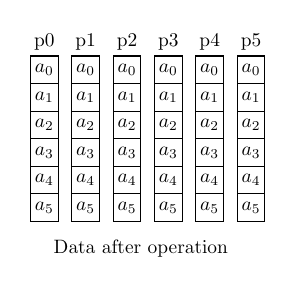
\begin{tikzpicture}[scale=0.35, every node/.style={transform shape}]
		
		%//starting at (0,0)
		
		\draw (0,0) -- (0,6) -- (1,6) -- (1,0) -- cycle;
		\foreach \x in {0,1,2,3,4, 5, 6}
		\draw (0,\x) -- (1,\x);
		
		\foreach \x/\val in {0/$a_5$,1/$a_4$,2/$a_3$,3/$a_2$,4/$a_1$, 5/$a_0$}
		\node [scale=2] at (0.5, 0.5 + \x) {\val};
		
		\foreach \x in {0,1,2,3,4, 5}
		\node [scale=2] at (1.5*\x+0.5 , 6.5) {p\x};
		
		\def\xstep{1.5}
		
		\draw (\xstep+0,0) -- (\xstep+0,6) -- (\xstep+1,6) -- (\xstep+1,0) -- cycle;
		\foreach \x in {0,1,2,3,4, 5, 6}
		\draw (\xstep+0,\x) -- (\xstep+1,\x);
		
		\foreach \x/\val in {0/$a_5$,1/$a_4$,2/$a_3$,3/$a_2$,4/$a_1$, 5/$a_0$}
		\node [scale=2] at (\xstep+0.5, 0.5 + \x) {\val};
		
		\def\xstep{3}
		
		\draw (\xstep+0,0) -- (\xstep+0,6) -- (\xstep+1,6) -- (\xstep+1,0) -- cycle;
		\foreach \x in {0,1,2,3,4, 5, 6}
		\draw (\xstep+0,\x) -- (\xstep+1,\x);
		
		\foreach \x/\val in {0/$a_5$,1/$a_4$,2/$a_3$,3/$a_2$,4/$a_1$, 5/$a_0$}
		\node [scale=2] at (\xstep+0.5, 0.5 + \x) {\val};
		
		
		\def\xstep{4.5}
		
		\draw (\xstep+0,0) -- (\xstep+0,6) -- (\xstep+1,6) -- (\xstep+1,0) -- cycle;
		\foreach \x in {0,1,2,3,4, 5, 6}
		\draw (\xstep+0,\x) -- (\xstep+1,\x);
		
		\foreach \x/\val in {0/$a_5$,1/$a_4$,2/$a_3$,3/$a_2$,4/$a_1$, 5/$a_0$}
		\node [scale=2] at (\xstep+0.5, 0.5 + \x) {\val};
		
		\def\xstep{6}
		
		\draw (\xstep+0,0) -- (\xstep+0,6) -- (\xstep+1,6) -- (\xstep+1,0) -- cycle;
		\foreach \x in {0,1,2,3,4, 5, 6}
		\draw (\xstep+0,\x) -- (\xstep+1,\x);
		
		\foreach \x/\val in {0/$a_5$,1/$a_4$,2/$a_3$,3/$a_2$,4/$a_1$, 5/$a_0$}
		\node [scale=2] at (\xstep+0.5, 0.5 + \x) {\val};
		
		\def\xstep{7.5}
		
		\draw (\xstep+0,0) -- (\xstep+0,6) -- (\xstep+1,6) -- (\xstep+1,0) -- cycle;
		\foreach \x in {0,1,2,3,4, 5, 6}
		\draw (\xstep+0,\x) -- (\xstep+1,\x);
		
		\foreach \x/\val in {0/$a_5$,1/$a_4$,2/$a_3$,3/$a_2$,4/$a_1$, 5/$a_0$}
		\node [scale=2] at (\xstep+0.5, 0.5 + \x) {\val};
		
		\node [scale=2] at (4, -1) {$\textnormal{Data after operation}$};
		\end{tikzpicture}
	\end{center}
\end{minipage}
\vfill
\begin{block}{Ring algorithm}
	\begin{itemize}
		\item Takes total $P-1$ steps
		\item In each step, process $i$ sends its contribution to process $i + 1$ and receives the contribution from process $i- 1$
		\item $T_{ring} = (P-1)\alpha + \left(\frac{P-1}{P}\right)n\beta$
		\item $n$ is the total amount of data gathered on each processor 
	\end{itemize}
\end{block}
\end{frame}
\begin{frame}{Recursive doubling algorithm for Allgather}
	\begin{minipage}{0.45\linewidth}
	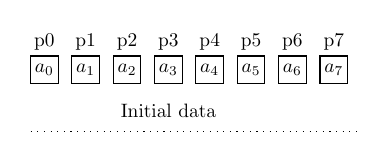
\begin{tikzpicture}[scale=0.35, every node/.style={transform shape}]
	\foreach \x in {0,1,2,3,4,5, 6, 7}
	{
		\draw (1.5*\x, 0) -- ++(1, 0) -- ++(0,1) -- ++(-1,0) -- cycle;
		\node [scale=2] at (1.5*\x+0.5, 0.5) {$a_\x$};
	}
	
	
	\foreach \x in {0,1,2,3,4,5,6,7}
	\node [scale=2] at (1.5*\x+0.5 , 1.5) {p\x};
	
	\node [scale=2] at (5, -1) {$\textnormal{Initial data}$};
	
	\draw [dotted] (0,-1.75) -- (12,-1.75);
	\path (0,-2) -- (12,-2);
	\end{tikzpicture}
	
	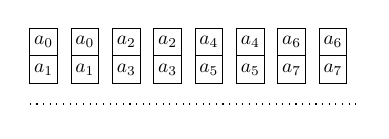
\begin{tikzpicture}[scale=0.35, every node/.style={transform shape}]
\def\xstep{0}
 		\draw (1.5*\xstep, 0) -- ++(1, 0) -- ++(0,1) -- ++(-1,0) -- cycle;
 		\draw (1.5*\xstep, 1) -- ++(1, 0) -- ++(0,1) -- ++(-1,0) -- cycle;
 		\node [scale=2] at (1.5*\xstep+0.5, 0.5) {$a_1$};
 		\node [scale=2] at (1.5*\xstep+0.5, 1+0.5) {$a_0$};
\def\xstep{1}
 		\draw (1.5*\xstep, 0) -- ++(1, 0) -- ++(0,1) -- ++(-1,0) -- cycle;
 		\draw (1.5*\xstep, 1) -- ++(1, 0) -- ++(0,1) -- ++(-1,0) -- cycle;
 		\node [scale=2] at (1.5*\xstep+0.5, 0.5) {$a_1$};
 		\node [scale=2] at (1.5*\xstep+0.5, 1+0.5) {$a_0$};
 		
\def\xstep{2}
 		\draw (1.5*\xstep, 0) -- ++(1, 0) -- ++(0,1) -- ++(-1,0) -- cycle;
 		\draw (1.5*\xstep, 1) -- ++(1, 0) -- ++(0,1) -- ++(-1,0) -- cycle;
 		\node [scale=2] at (1.5*\xstep+0.5, 0.5) {$a_3$};
 		\node [scale=2] at (1.5*\xstep+0.5, 1+0.5) {$a_2$};
 		
\def\xstep{3}
 		\draw (1.5*\xstep, 0) -- ++(1, 0) -- ++(0,1) -- ++(-1,0) -- cycle;
 		\draw (1.5*\xstep, 1) -- ++(1, 0) -- ++(0,1) -- ++(-1,0) -- cycle;
 		\node [scale=2] at (1.5*\xstep+0.5, 0.5) {$a_3$};
 		\node [scale=2] at (1.5*\xstep+0.5, 1+0.5) {$a_2$};
 		
 		\def\xstep{4}
 		\draw (1.5*\xstep, 0) -- ++(1, 0) -- ++(0,1) -- ++(-1,0) -- cycle;
 		\draw (1.5*\xstep, 1) -- ++(1, 0) -- ++(0,1) -- ++(-1,0) -- cycle;
 		\node [scale=2] at (1.5*\xstep+0.5, 0.5) {$a_5$};
 		\node [scale=2] at (1.5*\xstep+0.5, 1+0.5) {$a_4$};
 		
 		\def\xstep{5}
 		\draw (1.5*\xstep, 0) -- ++(1, 0) -- ++(0,1) -- ++(-1,0) -- cycle;
 		\draw (1.5*\xstep, 1) -- ++(1, 0) -- ++(0,1) -- ++(-1,0) -- cycle;
 		\node [scale=2] at (1.5*\xstep+0.5, 0.5) {$a_5$};
 		\node [scale=2] at (1.5*\xstep+0.5, 1+0.5) {$a_4$};
 		
 		\def\xstep{6}
 		\draw (1.5*\xstep, 0) -- ++(1, 0) -- ++(0,1) -- ++(-1,0) -- cycle;
 		\draw (1.5*\xstep, 1) -- ++(1, 0) -- ++(0,1) -- ++(-1,0) -- cycle;
 		\node [scale=2] at (1.5*\xstep+0.5, 0.5) {$a_7$};
 		\node [scale=2] at (1.5*\xstep+0.5, 1+0.5) {$a_6$};
 		
 		\def\xstep{7}
 		\draw (1.5*\xstep, 0) -- ++(1, 0) -- ++(0,1) -- ++(-1,0) -- cycle;
 		\draw (1.5*\xstep, 1) -- ++(1, 0) -- ++(0,1) -- ++(-1,0) -- cycle;
 		\node [scale=2] at (1.5*\xstep+0.5, 0.5) {$a_7$};
 		\node [scale=2] at (1.5*\xstep+0.5, 1+0.5) {$a_6$};
	
	\draw [dotted] (0,-0.75) -- (12,-0.75);
	\path (0,-1) -- (12, -1);
	\end{tikzpicture}
	
	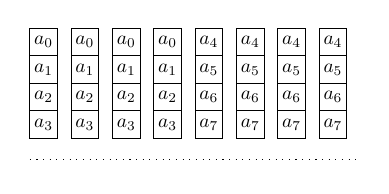
\begin{tikzpicture}[scale=0.35, every node/.style={transform shape}]
	\def\xstep{0}
	\foreach \x in {0,1,2,3}
	\draw (1.5*\xstep, \x) -- ++(1, 0) -- ++(0,1) -- ++(-1,0) -- cycle;

	
	\node [scale=2] at (1.5*\xstep+0.5, 0.5) {$a_3$};
	\node [scale=2] at (1.5*\xstep+0.5, 1+0.5) {$a_2$};
	\node [scale=2] at (1.5*\xstep+0.5, 2+0.5) {$a_1$};
	\node [scale=2] at (1.5*\xstep+0.5, 3+0.5) {$a_0$};
	
	\def\xstep{1}
	\foreach \x in {0,1,2,3}
	\draw (1.5*\xstep, \x) -- ++(1, 0) -- ++(0,1) -- ++(-1,0) -- cycle;
	
	\node [scale=2] at (1.5*\xstep+0.5, 0.5) {$a_3$};
	\node [scale=2] at (1.5*\xstep+0.5, 1+0.5) {$a_2$};
	\node [scale=2] at (1.5*\xstep+0.5, 2+0.5) {$a_1$};
	\node [scale=2] at (1.5*\xstep+0.5, 3+0.5) {$a_0$};
	

	\def\xstep{2}
	\foreach \x in {0,1,2,3}
	\draw (1.5*\xstep, \x) -- ++(1, 0) -- ++(0,1) -- ++(-1,0) -- cycle;
	
	\node [scale=2] at (1.5*\xstep+0.5, 0.5) {$a_3$};
	\node [scale=2] at (1.5*\xstep+0.5, 1+0.5) {$a_2$};
	\node [scale=2] at (1.5*\xstep+0.5, 2+0.5) {$a_1$};
	\node [scale=2] at (1.5*\xstep+0.5, 3+0.5) {$a_0$};
	
	\def\xstep{3}
	\foreach \x in {0,1,2,3}
	\draw (1.5*\xstep, \x) -- ++(1, 0) -- ++(0,1) -- ++(-1,0) -- cycle;
	
	\node [scale=2] at (1.5*\xstep+0.5, 0.5) {$a_3$};
	\node [scale=2] at (1.5*\xstep+0.5, 1+0.5) {$a_2$};
	\node [scale=2] at (1.5*\xstep+0.5, 2+0.5) {$a_1$};
	\node [scale=2] at (1.5*\xstep+0.5, 3+0.5) {$a_0$};
	
	
	\def\xstep{4}
	\foreach \x in {0,1,2,3}
	\draw (1.5*\xstep, \x) -- ++(1, 0) -- ++(0,1) -- ++(-1,0) -- cycle;
	
	\node [scale=2] at (1.5*\xstep+0.5, 0.5) {$a_7$};
	\node [scale=2] at (1.5*\xstep+0.5, 1+0.5) {$a_6$};
	\node [scale=2] at (1.5*\xstep+0.5, 2+0.5) {$a_5$};
	\node [scale=2] at (1.5*\xstep+0.5, 3+0.5) {$a_4$};
	
	\def\xstep{5}
	\foreach \x in {0,1,2,3}
	\draw (1.5*\xstep, \x) -- ++(1, 0) -- ++(0,1) -- ++(-1,0) -- cycle;
	
	\node [scale=2] at (1.5*\xstep+0.5, 0.5) {$a_7$};
	\node [scale=2] at (1.5*\xstep+0.5, 1+0.5) {$a_6$};
	\node [scale=2] at (1.5*\xstep+0.5, 2+0.5) {$a_5$};
	\node [scale=2] at (1.5*\xstep+0.5, 3+0.5) {$a_4$};
	
	

	
	\def\xstep{6}
	\foreach \x in {0,1,2,3}
	\draw (1.5*\xstep, \x) -- ++(1, 0) -- ++(0,1) -- ++(-1,0) -- cycle;
	
	\node [scale=2] at (1.5*\xstep+0.5, 0.5) {$a_7$};
	\node [scale=2] at (1.5*\xstep+0.5, 1+0.5) {$a_6$};
	\node [scale=2] at (1.5*\xstep+0.5, 2+0.5) {$a_5$};
	\node [scale=2] at (1.5*\xstep+0.5, 3+0.5) {$a_4$};
	
	
	\def\xstep{7}
	\foreach \x in {0,1,2,3}
	\draw (1.5*\xstep, \x) -- ++(1, 0) -- ++(0,1) -- ++(-1,0) -- cycle;
	
	\node [scale=2] at (1.5*\xstep+0.5, 0.5) {$a_7$};
	\node [scale=2] at (1.5*\xstep+0.5, 1+0.5) {$a_6$};
	\node [scale=2] at (1.5*\xstep+0.5, 2+0.5) {$a_5$};
	\node [scale=2] at (1.5*\xstep+0.5, 3+0.5) {$a_4$};
	
	\draw [dotted] (0,-0.75) -- (12,-0.75);
	\path (0,-1) -- (12, -1);
	\end{tikzpicture}
	
	
	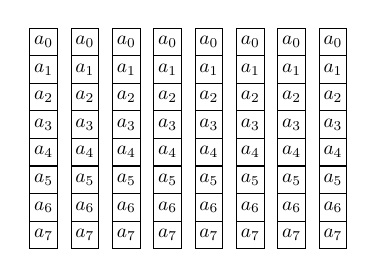
\begin{tikzpicture}[scale=0.35, every node/.style={transform shape}]

	\foreach \xstep in {0,1,2,3, 4, 5, 6, 7}
	\foreach \x in {0,1,2,3, 4, 5, 6, 7}
	{
	\draw (1.5*\xstep, \x) -- ++(1, 0) -- ++(0,1) -- ++(-1,0) -- cycle;
	\node [scale=2] at (1.5*\xstep+0.5, 7.5-\x) {$a_\x$};
	}
	
	\end{tikzpicture}
	\end{minipage}
	\begin{minipage}{0.525\linewidth}
	\begin{itemize}
		\item Assume $P$ is a perfect power of $2$
		\item In each step $k(0\le k <\lg P)$, processes that are at $2^k$ distance exchange their data
		\item $T_{rec\_dbl} = \lg P \alpha + \left(\frac{P-1}{P}\right)n\beta$ 
		\item Requires adaptation when $P$ is not a-power-of-two  
	\end{itemize}
	\end{minipage}
\end{frame}





\begin{frame}{Bruck's algorithm for Allgather}	
\begin{minipage}{0.3\linewidth}
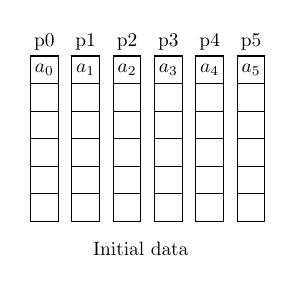
\begin{tikzpicture}[scale=0.35, every node/.style={transform shape}]

%//starting at (0,0)

\draw (0,0) -- (0,6) -- (1,6) -- (1,0) -- cycle;
\foreach \x in {0,1,2,3,4, 5, 6}
\draw (0,\x) -- (1,\x);


\foreach \x in {0,1,2,3,4, 5}
\node [scale=2] at (1.5*\x+0.5 , 6.5) {p\x};

\foreach \x/\val in {0/$ $,1/$ $,2/$ $,3/$ $,4/$ $, 5/$a_0$}
\node [scale=2] at (0.5, 0.5 + \x) {\val};

\def\xstep{1.5}

\draw (\xstep+0,0) -- (\xstep+0,6) -- (\xstep+1,6) -- (\xstep+1,0) -- cycle;
\foreach \x in {0,1,2,3,4, 5, 6}
\draw (\xstep+0,\x) -- (\xstep+1,\x);

\foreach \x/\val in {0/$ $,1/$ $,2/$ $,3/$ $,4/$ $, 5/$a_1$}
\node [scale=2] at (\xstep+0.5, 0.5 + \x) {\val};

\def\xstep{3}

\draw (\xstep+0,0) -- (\xstep+0,6) -- (\xstep+1,6) -- (\xstep+1,0) -- cycle;
\foreach \x in {0,1,2,3,4, 5, 6}
\draw (\xstep+0,\x) -- (\xstep+1,\x);

\foreach \x/\val in {0/$ $,1/$ $,2/$ $,3/$ $,4/$ $, 5/$a_2$}
\node [scale=2] at (\xstep+0.5, 0.5 + \x) {\val};


\def\xstep{4.5}

\draw (\xstep+0,0) -- (\xstep+0,6) -- (\xstep+1,6) -- (\xstep+1,0) -- cycle;
\foreach \x in {0,1,2,3,4, 5, 6}
\draw (\xstep+0,\x) -- (\xstep+1,\x);

\foreach \x/\val in {0/$ $,1/$ $,2/$ $,3/$ $,4/$ $, 5/$a_3$}
\node [scale=2] at (\xstep+0.5, 0.5 + \x) {\val};

\def\xstep{6}

\draw (\xstep+0,0) -- (\xstep+0,6) -- (\xstep+1,6) -- (\xstep+1,0) -- cycle;
\foreach \x in {0,1,2,3,4, 5, 6}
\draw (\xstep+0,\x) -- (\xstep+1,\x);

\foreach \x/\val in {0/$ $,1/$ $,2/$ $,3/$ $,4/$ $, 5/$a_4$}
\node [scale=2] at (\xstep+0.5, 0.5 + \x) {\val};

\def\xstep{7.5}

\draw (\xstep+0,0) -- (\xstep+0,6) -- (\xstep+1,6) -- (\xstep+1,0) -- cycle;
\foreach \x in {0,1,2,3,4, 5, 6}
\draw (\xstep+0,\x) -- (\xstep+1,\x);

\foreach \x/\val in {0/$ $,1/$ $,2/$ $,3/$ $,4/$ $, 5/$a_5$}
\node [scale=2] at (\xstep+0.5, 0.5 + \x) {\val};


\node [scale=2] at (4, -1) {$\textnormal{Initial data}$};
\end{tikzpicture}
\end{minipage}
\begin{minipage}{0.3\linewidth}
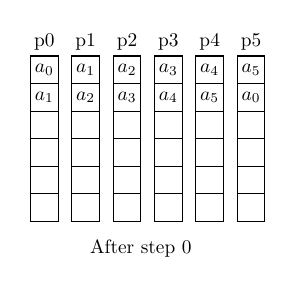
\begin{tikzpicture}[scale=0.35, every node/.style={transform shape}]

%//starting at (0,0)

\draw (0,0) -- (0,6) -- (1,6) -- (1,0) -- cycle;
\foreach \x in {0,1,2,3,4, 5, 6}
\draw (0,\x) -- (1,\x);

\foreach \x/\val in {0/$ $,1/$ $,2/$ $,3/$ $,4/$a_1$, 5/$a_0$}
\node [scale=2] at (0.5, 0.5 + \x) {\val};

\foreach \x in {0,1,2,3,4, 5}
\node [scale=2] at (1.5*\x+0.5 , 6.5) {p\x};

\def\xstep{1.5}

\draw (\xstep+0,0) -- (\xstep+0,6) -- (\xstep+1,6) -- (\xstep+1,0) -- cycle;
\foreach \x in {0,1,2,3,4, 5, 6}
\draw (\xstep+0,\x) -- (\xstep+1,\x);

\foreach \x/\val in {0/$ $,1/$ $,2/$ $,3/$ $,4/$a_2$, 5/$a_1$}
\node [scale=2] at (\xstep+0.5, 0.5 + \x) {\val};

\def\xstep{3}

\draw (\xstep+0,0) -- (\xstep+0,6) -- (\xstep+1,6) -- (\xstep+1,0) -- cycle;
\foreach \x in {0,1,2,3,4, 5, 6}
\draw (\xstep+0,\x) -- (\xstep+1,\x);

\foreach \x/\val in {0/$ $,1/$ $,2/$ $,3/$ $,4/$a_3$, 5/$a_2$}
\node [scale=2] at (\xstep+0.5, 0.5 + \x) {\val};


\def\xstep{4.5}

\draw (\xstep+0,0) -- (\xstep+0,6) -- (\xstep+1,6) -- (\xstep+1,0) -- cycle;
\foreach \x in {0,1,2,3,4, 5, 6}
\draw (\xstep+0,\x) -- (\xstep+1,\x);

\foreach \x/\val in {0/$ $,1/$ $,2/$ $,3/$ $,4/$a_4$, 5/$a_3$}
\node [scale=2] at (\xstep+0.5, 0.5 + \x) {\val};

\def\xstep{6}

\draw (\xstep+0,0) -- (\xstep+0,6) -- (\xstep+1,6) -- (\xstep+1,0) -- cycle;
\foreach \x in {0,1,2,3,4, 5, 6}
\draw (\xstep+0,\x) -- (\xstep+1,\x);

\foreach \x/\val in {0/$ $,1/$ $,2/$ $,3/$ $,4/$a_5$, 5/$a_4$}
\node [scale=2] at (\xstep+0.5, 0.5 + \x) {\val};

\def\xstep{7.5}

\draw (\xstep+0,0) -- (\xstep+0,6) -- (\xstep+1,6) -- (\xstep+1,0) -- cycle;
\foreach \x in {0,1,2,3,4, 5, 6}
\draw (\xstep+0,\x) -- (\xstep+1,\x);

\foreach \x/\val in {0/$ $,1/$ $,2/$ $,3/$ $,4/$a_0$, 5/$a_5$}
\node [scale=2] at (\xstep+0.5, 0.5 + \x) {\val};


\node [scale=2] at (4, -1) {$\textnormal{After step $0$}$};
\end{tikzpicture}
\end{minipage}
\begin{minipage}{0.3\linewidth}
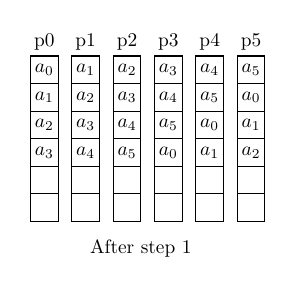
\begin{tikzpicture}[scale=0.35, every node/.style={transform shape}]

%//starting at (0,0)

\draw (0,0) -- (0,6) -- (1,6) -- (1,0) -- cycle;
\foreach \x in {0,1,2,3,4, 5, 6}
\draw (0,\x) -- (1,\x);

\foreach \x/\val in {0/$ $,1/$ $,2/$a_3$,3/$a_2$,4/$a_1$, 5/$a_0$}
\node [scale=2] at (0.5, 0.5 + \x) {\val};

\foreach \x in {0,1,2,3,4, 5}
\node [scale=2] at (1.5*\x+0.5 , 6.5) {p\x};

\def\xstep{1.5}

\draw (\xstep+0,0) -- (\xstep+0,6) -- (\xstep+1,6) -- (\xstep+1,0) -- cycle;
\foreach \x in {0,1,2,3,4, 5, 6}
\draw (\xstep+0,\x) -- (\xstep+1,\x);

\foreach \x/\val in {0/$ $,1/$ $,2/$a_4$,3/$a_3$,4/$a_2$, 5/$a_1$}
\node [scale=2] at (\xstep+0.5, 0.5 + \x) {\val};

\def\xstep{3}

\draw (\xstep+0,0) -- (\xstep+0,6) -- (\xstep+1,6) -- (\xstep+1,0) -- cycle;
\foreach \x in {0,1,2,3,4, 5, 6}
\draw (\xstep+0,\x) -- (\xstep+1,\x);

\foreach \x/\val in {0/$ $,1/$ $,2/$a_5$,3/$a_4$,4/$a_3$, 5/$a_2$}
\node [scale=2] at (\xstep+0.5, 0.5 + \x) {\val};


\def\xstep{4.5}

\draw (\xstep+0,0) -- (\xstep+0,6) -- (\xstep+1,6) -- (\xstep+1,0) -- cycle;
\foreach \x in {0,1,2,3,4, 5, 6}
\draw (\xstep+0,\x) -- (\xstep+1,\x);

\foreach \x/\val in {0/$ $,1/$ $,2/$a_0$,3/$a_5$,4/$a_4$, 5/$a_3$}
\node [scale=2] at (\xstep+0.5, 0.5 + \x) {\val};

\def\xstep{6}

\draw (\xstep+0,0) -- (\xstep+0,6) -- (\xstep+1,6) -- (\xstep+1,0) -- cycle;
\foreach \x in {0,1,2,3,4, 5, 6}
\draw (\xstep+0,\x) -- (\xstep+1,\x);

\foreach \x/\val in {0/$ $,1/$ $,2/$a_1$,3/$a_0$,4/$a_5$, 5/$a_4$}
\node [scale=2] at (\xstep+0.5, 0.5 + \x) {\val};

\def\xstep{7.5}

\draw (\xstep+0,0) -- (\xstep+0,6) -- (\xstep+1,6) -- (\xstep+1,0) -- cycle;
\foreach \x in {0,1,2,3,4, 5, 6}
\draw (\xstep+0,\x) -- (\xstep+1,\x);

\foreach \x/\val in {0/$ $,1/$ $,2/$a_2$,3/$a_1$,4/$a_0$, 5/$a_5$}
\node [scale=2] at (\xstep+0.5, 0.5 + \x) {\val};

\node [scale=2] at (4, -1) {$\textnormal{After step $1$}$};
\end{tikzpicture}
\end{minipage}


\vfill

\begin{minipage}{0.3\linewidth}
	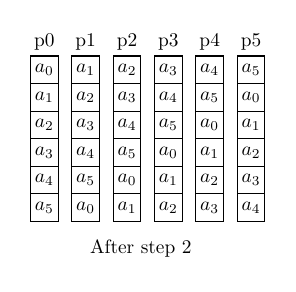
\begin{tikzpicture}[scale=0.35, every node/.style={transform shape}]
	
	%//starting at (0,0)
	
	\draw (0,0) -- (0,6) -- (1,6) -- (1,0) -- cycle;
	\foreach \x in {0,1,2,3,4, 5, 6}
	\draw (0,\x) -- (1,\x);
	
	\foreach \x/\val in {0/$a_5$,1/$a_4$,2/$a_3$,3/$a_2$,4/$a_1$, 5/$a_0$}
	\node [scale=2] at (0.5, 0.5 + \x) {\val};
	
	\foreach \x in {0,1,2,3,4, 5}
	\node [scale=2] at (1.5*\x+0.5 , 6.5) {p\x};
	
	\def\xstep{1.5}
	
	\draw (\xstep+0,0) -- (\xstep+0,6) -- (\xstep+1,6) -- (\xstep+1,0) -- cycle;
	\foreach \x in {0,1,2,3,4, 5, 6}
	\draw (\xstep+0,\x) -- (\xstep+1,\x);
	
	\foreach \x/\val in {0/$a_0$,1/$a_5$,2/$a_4$,3/$a_3$,4/$a_2$, 5/$a_1$}
	\node [scale=2] at (\xstep+0.5, 0.5 + \x) {\val};
	
	\def\xstep{3}
	
	\draw (\xstep+0,0) -- (\xstep+0,6) -- (\xstep+1,6) -- (\xstep+1,0) -- cycle;
	\foreach \x in {0,1,2,3,4, 5, 6}
	\draw (\xstep+0,\x) -- (\xstep+1,\x);
	
	\foreach \x/\val in {0/$a_1$,1/$a_0$,2/$a_5$,3/$a_4$,4/$a_3$, 5/$a_2$}
	\node [scale=2] at (\xstep+0.5, 0.5 + \x) {\val};
	
	
	\def\xstep{4.5}
	
	\draw (\xstep+0,0) -- (\xstep+0,6) -- (\xstep+1,6) -- (\xstep+1,0) -- cycle;
	\foreach \x in {0,1,2,3,4, 5, 6}
	\draw (\xstep+0,\x) -- (\xstep+1,\x);
	
	\foreach \x/\val in {0/$a_2$,1/$a_1$,2/$a_0$,3/$a_5$,4/$a_4$, 5/$a_3$}
	\node [scale=2] at (\xstep+0.5, 0.5 + \x) {\val};
	
	\def\xstep{6}
	
	\draw (\xstep+0,0) -- (\xstep+0,6) -- (\xstep+1,6) -- (\xstep+1,0) -- cycle;
	\foreach \x in {0,1,2,3,4, 5, 6}
	\draw (\xstep+0,\x) -- (\xstep+1,\x);
	
	\foreach \x/\val in {0/$a_3$,1/$a_2$,2/$a_1$,3/$a_0$,4/$a_5$, 5/$a_4$}
	\node [scale=2] at (\xstep+0.5, 0.5 + \x) {\val};
	
	\def\xstep{7.5}
	
	\draw (\xstep+0,0) -- (\xstep+0,6) -- (\xstep+1,6) -- (\xstep+1,0) -- cycle;
	\foreach \x in {0,1,2,3,4, 5, 6}
	\draw (\xstep+0,\x) -- (\xstep+1,\x);
	
	\foreach \x/\val in {0/$a_4$,1/$a_3$,2/$a_2$,3/$a_1$,4/$a_0$, 5/$a_5$}
	\node [scale=2] at (\xstep+0.5, 0.5 + \x) {\val};
	
	\node [scale=2] at (4, -1) {$\textnormal{After step $2$}$};
	\end{tikzpicture}
\end{minipage}
\begin{minipage}{0.3\linewidth}
	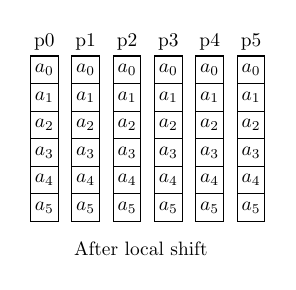
\begin{tikzpicture}[scale=0.35, every node/.style={transform shape}]
	
	%//starting at (0,0)
	
	\draw (0,0) -- (0,6) -- (1,6) -- (1,0) -- cycle;
	\foreach \x in {0,1,2,3,4, 5, 6}
	\draw (0,\x) -- (1,\x);
	
	\foreach \x/\val in {0/$a_5$,1/$a_4$,2/$a_3$,3/$a_2$,4/$a_1$, 5/$a_0$}
	\node [scale=2] at (0.5, 0.5 + \x) {\val};
	
	\foreach \x in {0,1,2,3,4, 5}
	\node [scale=2] at (1.5*\x+0.5 , 6.5) {p\x};
	
	\def\xstep{1.5}
	
	\draw (\xstep+0,0) -- (\xstep+0,6) -- (\xstep+1,6) -- (\xstep+1,0) -- cycle;
	\foreach \x in {0,1,2,3,4, 5, 6}
	\draw (\xstep+0,\x) -- (\xstep+1,\x);
	
	\foreach \x/\val in {0/$a_5$,1/$a_4$,2/$a_3$,3/$a_2$,4/$a_1$, 5/$a_0$}
	\node [scale=2] at (\xstep+0.5, 0.5 + \x) {\val};
	
	\def\xstep{3}
	
	\draw (\xstep+0,0) -- (\xstep+0,6) -- (\xstep+1,6) -- (\xstep+1,0) -- cycle;
	\foreach \x in {0,1,2,3,4, 5, 6}
	\draw (\xstep+0,\x) -- (\xstep+1,\x);
	
	\foreach \x/\val in {0/$a_5$,1/$a_4$,2/$a_3$,3/$a_2$,4/$a_1$, 5/$a_0$}
	\node [scale=2] at (\xstep+0.5, 0.5 + \x) {\val};
	
	
	\def\xstep{4.5}
	
	\draw (\xstep+0,0) -- (\xstep+0,6) -- (\xstep+1,6) -- (\xstep+1,0) -- cycle;
	\foreach \x in {0,1,2,3,4, 5, 6}
	\draw (\xstep+0,\x) -- (\xstep+1,\x);
	
	\foreach \x/\val in {0/$a_5$,1/$a_4$,2/$a_3$,3/$a_2$,4/$a_1$, 5/$a_0$}
	\node [scale=2] at (\xstep+0.5, 0.5 + \x) {\val};
	
	\def\xstep{6}
	
	\draw (\xstep+0,0) -- (\xstep+0,6) -- (\xstep+1,6) -- (\xstep+1,0) -- cycle;
	\foreach \x in {0,1,2,3,4, 5, 6}
	\draw (\xstep+0,\x) -- (\xstep+1,\x);
	
	\foreach \x/\val in {0/$a_5$,1/$a_4$,2/$a_3$,3/$a_2$,4/$a_1$, 5/$a_0$}
	\node [scale=2] at (\xstep+0.5, 0.5 + \x) {\val};
	
	\def\xstep{7.5}
	
	\draw (\xstep+0,0) -- (\xstep+0,6) -- (\xstep+1,6) -- (\xstep+1,0) -- cycle;
	\foreach \x in {0,1,2,3,4, 5, 6}
	\draw (\xstep+0,\x) -- (\xstep+1,\x);
	
	\foreach \x/\val in {0/$a_5$,1/$a_4$,2/$a_3$,3/$a_2$,4/$a_1$, 5/$a_0$}
	\node [scale=2] at (\xstep+0.5, 0.5 + \x) {\val};
	
	\node [scale=2] at (4, -1) {$\textnormal{After local shift}$};
	\end{tikzpicture}
\end{minipage}

\vfill

\begin{itemize}
	\item $T_{bruck} = \lceil \lg P \rceil \alpha + \frac{P-1}{P}n\beta$
	\item {\small In each step $k (0\le k < \lceil \lg P \rceil)$, process $i$ sends data to process $(i-2^k) \% P$ and receives data from process $(i+2^k) \% P$}
\end{itemize}
\end{frame}

\begin{frame}{Broadcast}
It broadcasts $n$ words from the root to all processes.
\smallskip
	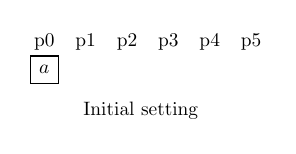
\begin{tikzpicture}[scale=0.35, every node/.style={transform shape}]
	
	%//starting at (0,0)
	
%
		\draw (1.5*0, 0) -- ++(1, 0) -- ++(0,1) -- ++(-1,0) -- cycle;
		\node [scale=2] at (1.5*0+0.5, 0.5) {$a$};
	
	
	\foreach \x in {0,1,2,3,4, 5}
	\node [scale=2] at (1.5*\x+0.5 , 1.5) {p\x};
	
	\node [scale=2] at (4, -1) {$\textnormal{Initial setting}$};
	\end{tikzpicture}$\qquad\qquad$
	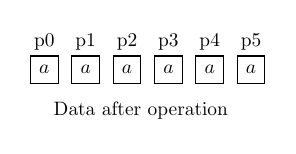
\begin{tikzpicture}[scale=0.35, every node/.style={transform shape}]
	
	%//starting at (0,0)
	
	\foreach \x in {0,1,2,3,4, 5}
	{
		\draw (1.5*\x, 0) -- ++(1, 0) -- ++(0,1) -- ++(-1,0) -- cycle;
		\node [scale=2] at (1.5*\x+0.5, 0.5) {$a$};
	}
	
	
	\foreach \x in {0,1,2,3,4, 5}
	\node [scale=2] at (1.5*\x+0.5 , 1.5) {p\x};
	
	\node [scale=2] at (4, -1) {$\textnormal{Data after operation}$};
	\end{tikzpicture}
\begin{block}{Bionomial tree algorithm}
	In the first step, the root sends data to process $(root +\frac{P}{2})$. This process and the root then act as new roots and recursively continue this algorithm.
	
	\begin{minipage}{0.56\linewidth}
		\begin{center}
	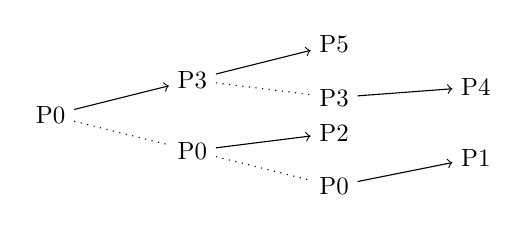
\begin{tikzpicture}[scale=0.45, every node/.style={transform shape}]
		\node (step1p0) [scale=2] at (0,2) {P0};
		\node (step2p0) [scale=2] at (4,1) {P0};
		\node (step2p3) [scale=2] at (4,3) {P3};
		
		\draw [dotted] (step1p0) -- (step2p0);
		\draw [->] (step1p0) -- (step2p3);
		
		\node (step3p0) [scale=2] at (8,0) {P0};
		\node (step3p2) [scale=2] at (8,1.5) {P2};
		\node (step3p3) [scale=2] at (8,2.5) {P3};
		\node (step3p5) [scale=2] at (8,4) {P5};
		
		\draw [dotted] (step2p0) -- (step3p0);
		\draw [dotted] (step2p3) -- (step3p3);
		\draw [->] (step2p3) -- (step3p5);
		\draw [->] (step2p0) -- (step3p2);
		
		
		\node (step4p1) [scale=2] at (12,0.8) {P1};
		\node (step4p4) [scale=2] at (12,2.8) {P4};
		
		\draw [->] (step3p0) -- (step4p1);
		\draw [->] (step3p3) -- (step4p4);
		
	\end{tikzpicture}
	\end{center}
	\end{minipage}\hfill
	\begin{minipage}{0.4\linewidth}
	\begin{itemize}
		\item $T_{tree}=\lceil\lg P \rceil (\alpha + n\beta)$
	\end{itemize}
	\end{minipage}		
\end{block}	

Alternative approach: Scatter + Allgather
\end{frame}

\begin{frame}{All-to-All}	
	\begin{minipage}{0.45\linewidth}
		\begin{center}
			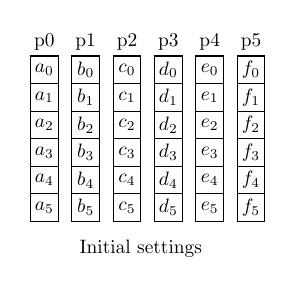
\begin{tikzpicture}[scale=0.35, every node/.style={transform shape}]
			\foreach \xstep/\val in {0/a,1/b,2/c,3/d, 4/e, 5/f}
			\foreach \x in {0,1,2,3, 4, 5}
			{
				\draw (1.5*\xstep, \x) -- ++(1, 0) -- ++(0,1) -- ++(-1,0) -- cycle;
				\node [scale=2] at (1.5*\xstep+0.5, 5.5-\x) {$\val_\x$};
			}
			
			\foreach \x in {0,1,2,3,4, 5}
			\node [scale=2] at (1.5*\x+0.5 , 6.5) {p\x};
			
			\node [scale=2] at (4, -1) {$\textnormal{Initial settings}$};
			\end{tikzpicture}	
		\end{center}
	\end{minipage}
	\begin{minipage}{0.45\linewidth}
		\begin{center}
			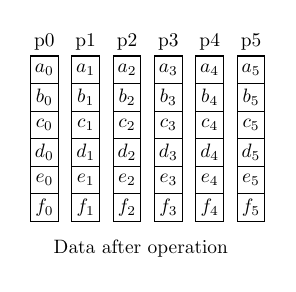
\begin{tikzpicture}[scale=0.35, every node/.style={transform shape}]

			\foreach \xstep in {0,1,2,3, 4, 5}
			\foreach \x/\val in {0/a,1/b,2/c,3/d, 4/e, 5/f}
			{
				\draw (1.5*\xstep, \x) -- ++(1, 0) -- ++(0,1) -- ++(-1,0) -- cycle;
				\node [scale=2] at (1.5*\xstep+0.5, 5.5-\x) {$\val_\xstep$};
			}
			
			\foreach \x in {0,1,2,3,4, 5}
			\node [scale=2] at (1.5*\x+0.5 , 6.5) {p\x};
			
			\node [scale=2] at (4, -1) {$\textnormal{Data after operation}$};
			\end{tikzpicture}
		\end{center}
	\end{minipage}
\begin{block}{Algorithm by Thakur et al.}
	\begin{itemize}
		\item In each step $k (1\le k < P)$, process $i$ receives data from process $(i-k)\%P$ and send data to process $(i+k)\%P$
		\item $T=(P-1)\alpha + \frac{P-1}{P}n\beta$
		\item $n$ is the total amount of data on any process in the beginning or end
	\end{itemize}
\end{block}
\end{frame}
\begin{frame}{Reduce-Scatter}	\begin{minipage}{0.45\linewidth}
		\vspace*{-0.15cm}
		\begin{center}
			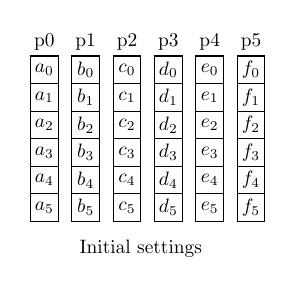
\begin{tikzpicture}[scale=0.35, every node/.style={transform shape}]
			\foreach \xstep/\val in {0/a,1/b,2/c,3/d, 4/e, 5/f}
			\foreach \x in {0,1,2,3, 4, 5}
			{
				\draw (1.5*\xstep, \x) -- ++(1, 0) -- ++(0,1) -- ++(-1,0) -- cycle;
				\node [scale=2] at (1.5*\xstep+0.5, 5.5-\x) {$\val_\x$};
			}
			
			\foreach \x in {0,1,2,3,4, 5}
			\node [scale=2] at (1.5*\x+0.5 , 6.5) {p\x};
			
			\node [scale=2] at (4, -1) {$\textnormal{Initial settings}$};
			\end{tikzpicture}	
		\end{center}
	\end{minipage}
	\begin{minipage}{0.45\linewidth}
		\begin{center}
			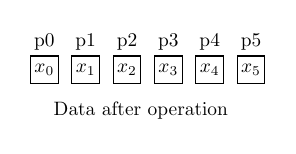
\begin{tikzpicture}[scale=0.35, every node/.style={transform shape}]
			
			\foreach \x in {0,1,2,3, 4, 5}
			{
				\draw (1.5*\x, 0) -- ++(1, 0) -- ++(0,1) -- ++(-1,0) -- cycle;
				\node [scale=2] at (1.5*\x+0.5, 0.5) {$x_\x$};
			}
			
			\foreach \x in {0,1,2,3,4, 5}
			\node [scale=2] at (1.5*\x+0.5 , 1.5) {p\x};
			
			\node [scale=2] at (4, -1) {$\textnormal{Data after operation}$};
			\end{tikzpicture}
		\end{center}\vspace*{-0.35cm}
	$x_i=\textnormal{Reduce}(a_i,b_i,c_i,d_i,e_i)$\\
	{\small Each process has $n$ amount of data in the beginning.} 
	\end{minipage}
\vspace*{-0.25cm}
\begin{block}{Recursive halving algorithm (Assuming $P$ is a perfect power of $2$)}
	\vspace*{-0.15cm}{\small\begin{itemize}
		\item Analogous to the recursive-doubling algorithm for Allgather
		\item In each step $k(1\le k \le P)$, processes that are at $\frac{P}{2^k}$ distance
		exchange parts of their data
		\item Each process sends the data needed by all processes in the other half, receives the data needed by all processes in its own half
		\item $T_{rec\_half} = \lg P \alpha + \frac{P-1}{P} n \beta + \frac{P-1}{P} n \gamma$
		\item Requires adaptation when $P$ is not a power-of-two
	\end{itemize}}
\end{block}
\vspace*{-0.15cm}
\begin{block}{}
\vspace*{-0.25cm}{\small\begin{itemize}
	\item With an adaptation of Bruck's algorithm: $T_{bruck} = \lceil \lg P \rceil \alpha + \frac{P-1}{P} n \beta + \frac{P-1}{P} n \gamma$\vspace*{-0.1cm}
\end{itemize}}
\end{block}
\end{frame}
\begin{frame}{Reduce and Allreduce}
Each process has $n$ amount of data in the beginning.
\vfill
	\begin{block}{Reduce}
		\begin{itemize}
			\item With binomial tree algorithm, $T_{tree} = \lceil\lg P \rceil (\alpha+n\beta+n\gamma)$
			\item With Reduce-Scatter(Bruck's algorithm) + Gather(Binomial tree), $T=2\lceil\lg P \rceil \alpha +  2\frac{P-1}{P} n \beta + \frac{P-1}{P} n \gamma$
		\end{itemize}
	\end{block}
\vfill
	\begin{block}{Allreduce}
	\begin{itemize}
	\item With Reduce-Scatter(Bruck's algorithm) + Allgather(Bruck's algorithm), $T=2\lceil\lg P \rceil \alpha +  2\frac{P-1}{P} n \beta + \frac{P-1}{P} n \gamma$
	\end{itemize}
	\end{block}
\vfill
\end{frame}
\begin{frame}
\begin{thebibliography}{10}
	\bibitem{thakur05}
	\alert{R. Thakur, R. Rabenseifner, and W. Gropp (2005).}
	\newblock  {Optimization of Collective Communication Operations in MPICH}
	\newblock {\em Int. J. High Perform. Comput. Appl. 19, 1 (February  2005), 49–66}.
	
	\bibitem{chan04}
	\alert{E. W. Chan, M. F. Heimlich, A. Purkayastha and R. A. van de Geijn}
	\newblock {On Optimizing Collective Communication}
	\newblock {IEEE International Conference on Cluster Computing, San Diego, CA, USA, 2004, pp. 145-155}.
\end{thebibliography}
\end{frame}
\end{document} 